\documentclass{article}
\usepackage{graphicx}
\graphicspath{ {Announcements/} }
\usepackage{hyperref}
\usepackage[margin=0.5in]{geometry}

\begin{document}

\section*{Changes to sfucsss Website}

\begin{enumerate}
	\item go to URL: \url{sfucsss.org/admin}
	\item login
	\item \textbf{Creating Front-Page announcement}
	\begin{itemize}
		\item Click on "Add"
		
		\includegraphics[scale=0.45]{Announcements-picture1.png}
		
	\end{itemize}
	\item \textbf{Modifying/Deleting existing Front-page announcement}
	\begin{itemize}
		\item Click on "Change"
		
		\includegraphics[scale=0.45]{Announcements-picture2.png}
 
	\end{itemize}
	\item \textbf{Adding a Category to the Website}
	
	Example Categories: \includegraphics[scale=0.45]{Categories-picture1.png}
	
	\begin{itemize}
		\item Click on "Add"
		
		\includegraphics[scale=0.45]{Categories-picture2.png}
		
	\end{itemize}
	\item \textbf{Modifying/Deleting existing category}
	\begin{itemize}
		\item Click on "Categories"
		
		\includegraphics[scale=0.45]{Categories-picture3.png}
		
	\end{itemize}
	\item \textbf{To add Any Pages to the Website}
	\begin{itemize}
		\item Click on "Add"
		
		\includegraphics[scale=0.45]{posts-picture1.png}
		
		\item Enter the following required information
		
		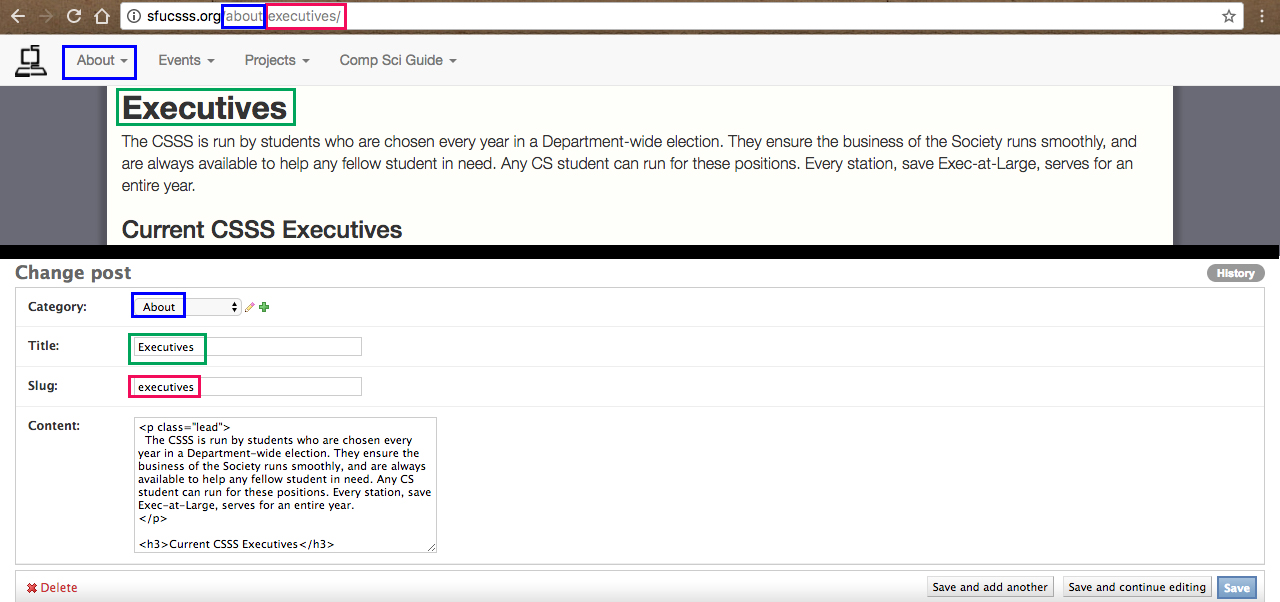
\includegraphics[scale=0.40]{Posts.jpg}
	\end{itemize}
	\item \textbf{To modify/delete any existing pages}
	\begin{itemize}
		\item Click on "Change"
		
		\includegraphics[scale=0.45]{posts-picture2.png}
		
	\end{itemize}
\end{enumerate}

		
\end{document}